\section{Motivation}

The previous chapter introduced robust MPC methods that explicitly account for bounded
disturbances in the controller design. In particular, we studied robust open-loop MPC,
constraint-tightening MPC, and tube MPC. In all those approaches, the controller is modified so
that the predicted trajectories contain safety margins against the effect of disturbances.\\

In this chapter we consider a different question. Suppose the real system is affected by noise,
but the controller ignores this fact and solves the standard nominal MPC problem. This is very
common in practice. Engineers often use a nominal model, implement MPC in receding horizon,
and rely on feedback and repeated re-optimization to compensate for small disturbances. The
question is then: can we say anything rigorous about this strategy?

We consider the noisy linear system
\[
    x(k+1)=Ax(k)+Bu(k)+w(k),
\]
where \(w(k)\) is an additive disturbance. Instead of designing a robust MPC controller, we solve
the nominal finite-horizon problem
\[
\begin{aligned}
    J^\star(x_0)
    =
    \min_U\quad
    &
    \sum_{i=0}^{N-1}\ell(x_i,u_i)+\ell_f(x_N)
    \\
    \text{subj. to}\quad
    &
    x_{i+1}=Ax_i+Bu_i,
    \qquad i=0,\ldots,N-1,
    \\
    &
    x_i\in\mathcal X,\qquad u_i\in\mathcal U,
    \qquad i=0,\ldots,N-1,
    \\
    &
    x_N\in\mathcal X_f,
    \\
    &
    x_0=x(k).
\end{aligned}
\]
The controller applies only the first element of the optimal input sequence:
\[
    u(k)=u_0^\star(x(k)).
\]
Since the plant is disturbed, the true closed-loop system is not the nominal one used in the
prediction. It is instead
\[
    x(k+1)=Ax(k)+Bu_0^\star(x(k))+w(k).
\]

\begin{theorembox}[Nominal MPC applied to a noisy system]
Nominal MPC ignores the disturbance in the prediction model, but the real closed-loop system is
\[
    x(k+1)=Ax(k)+Bu_0^\star(x(k))+w(k).
\]
Thus the controller is designed for the nominal dynamics, while the plant evolves according to
the disturbed dynamics.
\end{theorembox}

The main result is not a full robust constraint-satisfaction guarantee. Unlike tube MPC, nominal
MPC does not explicitly enforce tightened constraints, and therefore one cannot generally certify
that all constraints are satisfied for all disturbance realizations. However, under suitable
regularity assumptions, one can prove a weaker but important property: the closed-loop state
converges to a neighborhood of the origin whose size depends on the disturbance magnitude.
This is the idea of input-to-state stability.

\section{Nominal MPC with Noise}

\subsection{Ignoring the noise}

The nominal MPC problem assumes that the future states satisfy
\[
    x_{i+1}=Ax_i+Bu_i.
\]
The optimizer therefore computes a trajectory that is feasible and stabilizing for the nominal
model. But after applying the first input, the real system evolves as
\[
    x(k+1)=Ax(k)+Bu_0^\star(x(k))+w(k).
\]
Thus, even if the nominal successor
\[
    Ax(k)+Bu_0^\star(x(k))
\]
lies in the desired feasible region, the actual successor may be shifted by the disturbance.\\

This is precisely the situation that robust MPC was designed to avoid. In robust MPC, one
accounts for \(w(k)\) explicitly by tightening constraints or propagating uncertainty sets. In
nominal MPC, no such margin is introduced. Nevertheless, because MPC is implemented in
receding horizon, the controller will remeasure the disturbed state at the next time step and
solve a new optimization problem from there. This feedback effect may be enough to compensate
for small disturbances in many practical cases.

\subsection{Example: many disturbance realizations}

The behavior of nominal MPC under disturbances can be illustrated by simulating many
closed-loop trajectories with different disturbance realizations. The controller is the same in all
cases: it is the nominal MPC controller that pretends the noise is absent. The only difference
between the trajectories is the disturbance sequence acting on the real system.\\

In some simulations, all trajectories appear to move toward the origin and remain well behaved.
This suggests that nominal MPC can be robust in practice, at least for small disturbances and
suitable initial states. However, this observation alone is not a guarantee. Other initial states,
or other disturbance realizations, may lead to constraint violations or to poor closed-loop
behavior. The important point is therefore not only whether the controller works in a simulation,
but how to formalize the region in which it works.

\begin{figure}[!h]
    \centering

    \begin{subfigure}[t]{0.48\textwidth}
        \centering
        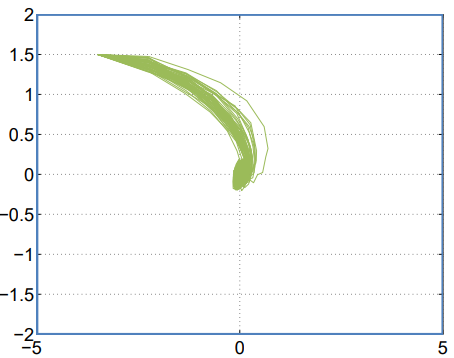
\includegraphics[width=\textwidth]{images/nominal_mpc_noise_example_1.png}
        \caption{For some initial conditions and disturbance realizations, nominal MPC appears
        to work well despite the noise.}
        \label{fig:nominal_mpc_noise_example_1}
    \end{subfigure}
    \hfill
    \begin{subfigure}[t]{0.48\textwidth}
        \centering
        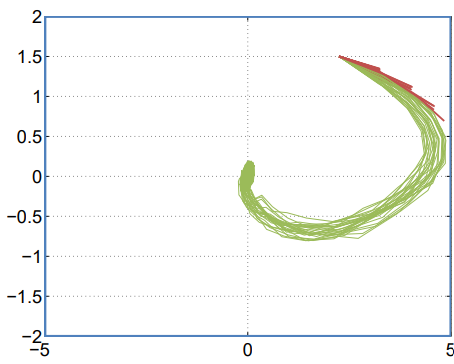
\includegraphics[width=\textwidth]{images/nominal_mpc_noise_example_2.png}
        \caption{For other initial conditions, the behavior is less certain: the same nominal MPC
        law may work for some disturbance realizations but not for all.}
        \label{fig:nominal_mpc_noise_example_2}
    \end{subfigure}

    \caption{Nominal MPC applied to a noisy system. The controller ignores the disturbance,
    while the closed-loop trajectories correspond to different noise realizations. The simulations
    may look acceptable, but they do not provide the same guarantees as robust MPC.}
    \label{fig:nominal_mpc_noise_examples}
\end{figure}

This example motivates the central question of the chapter. If we do not explicitly design a
robust controller, can we still prove that the closed-loop system remains bounded or converges
near the origin? The answer relies on the behavior of the nominal MPC value function under
small perturbations.

\section{What Happens to the Lyapunov Function?}

\subsection{Nominal Lyapunov decrease}

Recall the standard nominal MPC stability argument. Under the usual terminal ingredients, the
optimal cost
\[
    J^\star(x)
\]
acts as a Lyapunov function for the nominal closed-loop system
\[
    x^+=Ax+Bu^\star(x),
\]
where \(u^\star(x)\) denotes the first input selected by the nominal MPC controller. More
precisely, one obtains the decrease condition
\[
    J^\star(Ax+Bu^\star(x))-J^\star(x)
    \leq
    -\ell(x,u^\star(x)).
\]
This inequality says that the optimal value decreases along nominal closed-loop trajectories by
at least the stage cost. Since the stage cost is positive definite, this gives convergence to the
origin in the nominal case.

\begin{theorembox}[Nominal MPC Lyapunov decrease]
For the nominal closed-loop system
\[
    x^+=Ax+Bu^\star(x),
\]
the optimal value function satisfies
\[
    J^\star(Ax+Bu^\star(x))-J^\star(x)
    \leq
    -\ell(x,u^\star(x)).
\]
Thus \(J^\star\) is a Lyapunov function for the nominal closed loop.
\end{theorembox}

In the noisy case, however, the next state is not
\[
    Ax+Bu^\star(x),
\]
but
\[
    Ax+Bu^\star(x)+w.
\]
The question is therefore whether the Lyapunov decrease survives this perturbation.

\subsection{Perturbed Lyapunov decrease}

Assume that the optimal value function \(J^\star\) is Lipschitz continuous on the relevant
feasible set. This means that there exists a constant \(\gamma>0\) such that
\[
    |J^\star(x_1)-J^\star(x_2)|
    \leq
    \gamma\norm{x_1-x_2}
\]
for all states \(x_1,x_2\) in that set. Applying this property to the nominal successor and the
disturbed successor gives
\[
\begin{aligned}
&
\left|
J^\star(Ax+Bu^\star(x)+w)
-
J^\star(Ax+Bu^\star(x))
\right|
\\
&\qquad\leq
\gamma
\norm{
Ax+Bu^\star(x)+w
-
(Ax+Bu^\star(x))
}
=
\gamma\norm{w}.
\end{aligned}
\]
Thus the disturbance can increase the Lyapunov function, but the increase is bounded by a term
proportional to the disturbance size.\\

We can now estimate the change of \(J^\star\) along the disturbed closed loop:
\[
\begin{aligned}
&
J^\star(Ax+Bu^\star(x)+w)-J^\star(x)
\\
&=
J^\star(Ax+Bu^\star(x)+w)
-
J^\star(Ax+Bu^\star(x))
\\
&\qquad
+
J^\star(Ax+Bu^\star(x))
-
J^\star(x)
\\
&\leq
\gamma\norm{w}
-
\ell(x,u^\star(x)).
\end{aligned}
\]
Hence
\[
    J^\star(Ax+Bu^\star(x)+w)-J^\star(x)
    \leq
    -\ell(x,u^\star(x))+\gamma\norm{w}.
\]

\begin{theorembox}[Perturbed Lyapunov decrease]
If \(J^\star\) is Lipschitz continuous with constant \(\gamma\), then along the disturbed
closed-loop system
\[
    x^+=Ax+Bu^\star(x)+w
\]
one has
\[
    J^\star(x^+)-J^\star(x)
    \leq
    -\ell(x,u^\star(x))+\gamma\norm{w}.
\]
\end{theorembox}

This inequality explains the qualitative behavior of nominal MPC under bounded disturbances.
The negative term
\[
    -\ell(x,u^\star(x))
\]
becomes larger in magnitude when the state is far from the origin, while the positive term
\[
    \gamma\norm{w}
\]
is bounded by the size of the disturbance. Therefore, far from the origin the Lyapunov function
still decreases. Close to the origin, however, the nominal decrease becomes small and may be
balanced by the disturbance effect. The state then cannot be expected to converge exactly to
zero, but it can converge to a neighborhood of zero.

\section{Special Case: When Nominal MPC is Robust}

The previous argument depends on the Lipschitz continuity of the optimal value function. This
property is not automatic for arbitrary nonlinear MPC problems, but it holds in important
linear settings. In particular, if the nominal model is linear, the cost is linear or quadratic, and
the constraint sets are polytopes, then the finite-horizon optimal value function
\[
    V_N^\star(x)
\]
is Lipschitz continuous on the feasible set \(\mathcal X_N\).\\

This is consistent with the explicit MPC results discussed earlier. For linear MPC with
polyhedral constraints, the optimal control law and value function have a piecewise structure.
With linear costs, the value function is piecewise affine. With quadratic costs, the value
function is piecewise quadratic. On compact polytopic regions, these piecewise affine or
piecewise quadratic functions are Lipschitz continuous.

\begin{theorembox}[Lipschitz value function for linear nominal MPC]
If the model is linear, the constraints are polytopic, and the finite-horizon cost is linear or
quadratic, then the nominal MPC value function
\[
    V_N^\star(x)
\]
is Lipschitz continuous on the feasible set \(\mathcal X_N\).
\end{theorembox}

\begin{figure}[!h]
    \centering
    % Replace the file name with the corresponding slide/image file.
    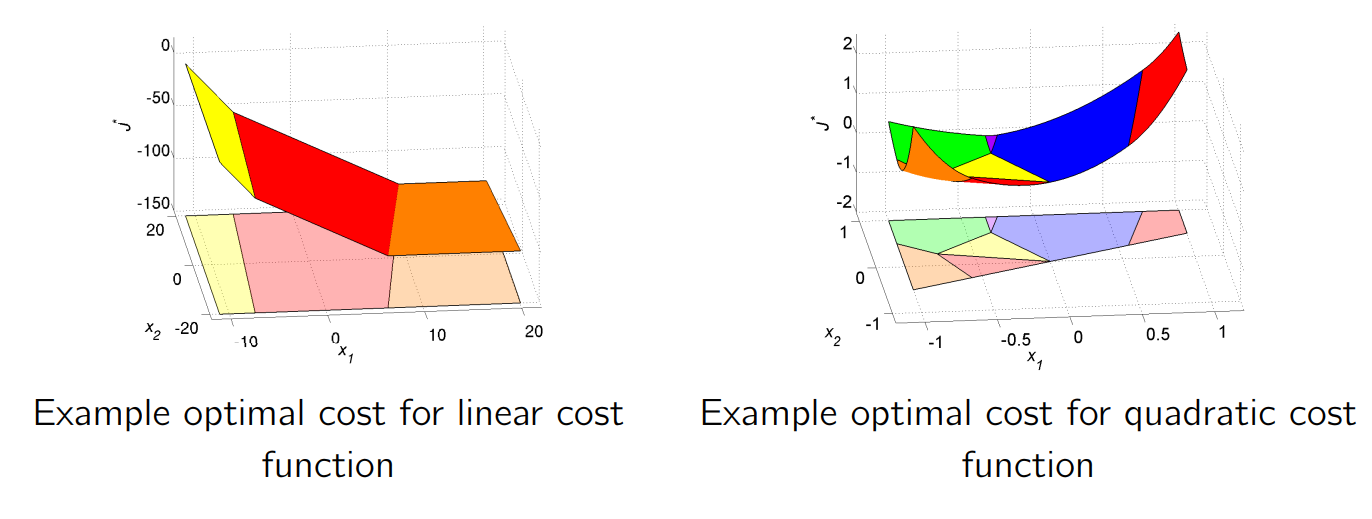
\includegraphics[width=0.78\textwidth]{images/nominal_mpc_value_function_lipschitz.png}
    \caption{Piecewise structure of the nominal MPC value function. For linear MPC with
    polytopic constraints, a linear cost leads to a piecewise affine value function, while a
    quadratic cost leads to a piecewise quadratic value function. On compact feasible regions,
    such functions are Lipschitz continuous.}
    \label{fig:nominal_mpc_value_function_lipschitz}
\end{figure}

This special case is important because it gives a rigorous explanation for why nominal MPC may
remain well behaved under small disturbances. The nominal Lyapunov decrease is not destroyed
completely by the disturbance; it is only perturbed by a bounded term.

\section{Input-to-State Stability Interpretation}

The perturbed Lyapunov inequality
\[
    J^\star(x^+)-J^\star(x)
    \leq
    -\ell(x,u^\star(x))+\gamma\norm{w}
\]
is the key to the input-to-state stability interpretation. In nominal asymptotic stability, the
Lyapunov function decreases monotonically to zero, and the state converges to the origin. With
persistent disturbances, the decrease is interrupted by the additive term depending on
\(\norm{w}\).\\

If the state is large, the stage cost \(\ell(x,u^\star(x))\) is large, and the Lyapunov function
decreases. As the state becomes smaller, the stage cost becomes smaller as well. Eventually, the
nominal decrease and the disturbance-induced increase balance each other. At that point, one
can no longer guarantee convergence closer to the origin. Instead, one guarantees convergence
to a set around the origin whose size depends on the maximum disturbance magnitude:
\[
    \max_{w\in\mathcal W}\norm{w}.
\]

\begin{theorembox}[Input-to-state stability intuition]
Nominal MPC applied to a disturbed system may still be input-to-state stable. The state is
driven toward the origin until the nominal Lyapunov decrease is balanced by the disturbance
effect. Therefore, the closed-loop state converges to a neighborhood of the origin whose size is
determined by the size of the disturbance.
\end{theorembox}

\begin{figure}[!h]
    \centering
    % Replace the file name with the corresponding slide/image file.
    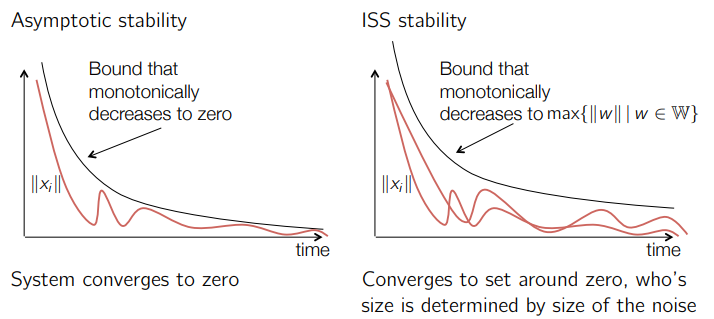
\includegraphics[width=0.76\textwidth]{images/input_to_state_stability_nominal_mpc.png}
    \caption{Comparison between asymptotic stability and input-to-state stability. In the
    disturbance-free case, the bound on the state decreases to zero. In the disturbed case, the
    state converges to a neighborhood of the origin, whose size depends on the disturbance
    magnitude.}
    \label{fig:iss_nominal_mpc}
\end{figure}

This is weaker than the guarantees obtained with robust constraint tightening or tube MPC. In
tube MPC, the invariant tube is explicitly constructed, and constraints are tightened to guarantee
robust satisfaction. For nominal MPC, the result is more qualitative: small disturbances may
lead only to small steady-state deviations, but the controller does not explicitly certify robust
constraint satisfaction for all states and all disturbances.

\section{Discussion}

The robustness of nominal MPC is both practically important and conceptually subtle. On the
one hand, nominal MPC is simple. It does not require the designer to know the disturbance set
\(\mathcal W\), and it often works well in practice. This is one reason why nominal MPC is so
widely used: repeated measurement and re-optimization already provide some disturbance
rejection.\\

On the other hand, nominal MPC does not provide the same guarantees as robust MPC. Since
the controller ignores the disturbance in the optimization problem, the feasible nominal
trajectory may lie close to the boundary of the constraints. A disturbance can then push the
real state outside the admissible set. Moreover, the region of attraction is difficult to
characterize. Some initial states may work for many disturbance realizations, while others may
fail for only a few.\\

Thus nominal MPC has a large apparent feasible set, because the optimization problem is easier
to satisfy. But this feasible set should not be confused with a robust feasible set. It contains
states from which the nominal problem has a solution, not necessarily states from which the real
disturbed closed loop is guaranteed to satisfy constraints for all time.

\begin{theorembox}[Nominal MPC versus robust MPC]
Nominal MPC may be robust in the sense of input-to-state stability, but it does not generally
provide robust constraint satisfaction. Robust MPC explicitly accounts for the disturbance,
whereas nominal MPC relies on feedback and repeated re-optimization.
\end{theorembox}

\section{Summary}

Nominal MPC for uncertain systems is based on a simple idea: ignore the noise in the prediction
model and rely on receding-horizon feedback to compensate for it. The nominal controller solves
\[
\begin{aligned}
    \min_U\quad
    &
    \sum_{i=0}^{N-1}\ell(x_i,u_i)+\ell_f(x_N)
    \\
    \text{subj. to}\quad
    &
    x_{i+1}=Ax_i+Bu_i,
    \\
    &
    x_i\in\mathcal X,\qquad u_i\in\mathcal U,
    \\
    &
    x_N\in\mathcal X_f,
\end{aligned}
\]
but the actual closed-loop system is
\[
    x(k+1)=Ax(k)+Bu_0^\star(x(k))+w(k).
\]

The main benefit of this approach is simplicity. No disturbance set \(\mathcal W\) is required,
the online optimization problem is the standard nominal MPC problem, and the method is often
effective in practice. The nominal feasible set may also be larger than the feasible set of robust
MPC methods, because no constraints are tightened.\\

The main limitation is the absence of explicit robust guarantees. It is difficult to determine the
true region of attraction, hard to tune the tradeoff between robustness and performance, and
constraint satisfaction cannot generally be guaranteed for all disturbance realizations. For
linear systems with polytopic constraints and linear or quadratic costs, the nominal MPC value
function is Lipschitz continuous, and this allows one to prove an input-to-state stability type
result:
\[
    J^\star(x^+)-J^\star(x)
    \leq
    -\ell(x,u^\star(x))+\gamma\norm{w}.
\]
Thus the system moves toward the origin until the nominal decrease is balanced by the
disturbance effect. The correct conclusion is convergence to a neighborhood of the origin, not
necessarily convergence to the origin itself.